\documentclass[11pt]{article}
\usepackage[top=2cm,bottom=2cm,left=1.5cm,right=1.5cm]{geometry}
%\geometry{landscape}                % Activate for for rotated page geometry
\usepackage[parfill]{parskip}    % Activate to begin paragraphs with an empty line rather than an indent
\usepackage{graphicx}
\usepackage{amssymb}
\usepackage{epstopdf}
\usepackage{amsmath}            
\usepackage{multirow}    
\usepackage{hyperref}
\usepackage{changepage}
\usepackage{lscape}
\usepackage{ulem}
\usepackage{multicol}
\usepackage{dashrule}
\usepackage[usenames,dvipsnames]{color}       
\usepackage{enumerate}
\newcommand{\urlwofont}[1]{\urlstyle{same}\url{#1}}
\newcommand{\degree}{\ensuremath{^\circ}}
\newcommand{\hl}[1]{\textbf{\underline{#1}}}



\DeclareGraphicsRule{.tif}{png}{.png}{`convert #1 `dirname #1`/`basename #1 .tif`.png}

\newenvironment{choices}{
\begin{enumerate}[(a)]
}{\end{enumerate}}

%\newcommand{\soln}[1]{\textcolor{MidnightBlue}{\textit{#1}}}	% delete #1 to get rid of solutions for handouts
\newcommand{\soln}[1]{ \vspace{1.35cm} }

%\newcommand{\solnMult}[1]{\textbf{\textcolor{MidnightBlue}{\textit{#1}}}}	% uncomment for solutions
\newcommand{\solnMult}[1]{ #1 }	% uncomment for handouts

\newcommand{\pts}[1]{ \textbf{{\footnotesize \textcolor{black}{(#1)}}} }	% uncomment for handouts
%\newcommand{\pts}[1]{ \textbf{{\footnotesize \textcolor{blue}{(#1)}}} }	% uncomment for handouts

\newcommand{\note}[1]{ \textbf{\textcolor{red}{[#1]}} }	% uncomment for handouts

\begin{document}

%

Dr \c{C}etinkaya-Rundel \hfill Sta 101 \\

\begin{center}
{\LARGE Sample MT2}
\end{center}

\begin{enumerate}

\item On March 23, 2012 SurveyUSA conducted a poll in Florida on the shooting of Trayvon Martin. The table below shows the distribution of political ideology of respondents and the degree to which they think the victim's race was a factor in this shooting. \\

\begin{center}
\begin{tabular}{r c c c | c}
  \hline
 			& conservative & moderate	& liberal 	& total \\ 
  \hline
not a factor 	& 64 			&  43 		& 17 		& 124 \\ 
small factor 	& 54			&  79 		& 13 		& 146 \\ 
major factor	& 80 			& 179 		& 99		& 358 \\
not sure		& 40 			& 44 			& 26 		& 110 \\
   \hline
total			& 238		& 345		& 155 	& 738 \\
   \hline
\end{tabular}
\end{center}

\vspace{0.25cm}

\begin{enumerate}

\item \pts{2} What are the cases in this survey, and how many cases are there?

\soln{Cases in this study are 738 randomly selected Florida residents.}

\item \pts{4} What are the variables in this study? Identify each variable as categorical or numerical.

\soln{Variable 1: political ideology (categorical) \\
Variable 2: degree to which the respondent thinks the victim's race was a major factor in this shooting (categorical, ordinal)}

\item \pts{2} Name \emph{one} inference method that is appropriate for examining the relationship between the variables in this study? Be specific.

\soln{Chi-squared test of independence.}

\item \pts{4} Write the hypotheses for testing for a relationship between these two variables. You can avoid notation and simply write the hypotheses in words.

\soln{$H_0$: Political ideology and the degree to which Florida residents think the victim's race was a major factor in this shooting are independent of each other. \\
$H_A$: Political ideology and the degree to which Florida residents think the victim's race was a major factor in this shooting are associated.
}
$\:$

\item \pts{3} If the variables in the study are not related, how many \emph{liberal} respondents would we expect to have responded ``not a factor"?

\soln{\[ E_{\text{not a factor, liberal}} = \frac{124 \times 155}{738} = 26.04 \approx 26 \]}
$\:$

\item \pts{2} The test statistic is calculated as 55.55. What is the p-value? Make sure to show all your work.

\soln{$df = (R - 1) \times (C - 1) = 3 \times 2 = 6$, p-value is less than 0.001.}

\item \pts{4} What is the conclusion of the hypothesis test at the 5\% significance level? Interpret your conclusion in the context of this question.

\soln{Reject $H_0$. The data provide convincing evidence that the political ideology and the degree to which Florida residents think the victim's race was a major factor in this shooting are associated.}

\end{enumerate}

%

\pagebreak

\item Researchers were interested in the effect of stents, devices put inside blood vessels that assist in patient recovery after cardiac events, as preventative devices for patients at risk of stroke. They randomly assigned 451 at risk patients to control and treatment groups. The 224 patients in the treatment group received a stent and aggressive medical management, including medications, management of risk factors, and help in lifestyle modification. The remaining 227 patients in the control group received aggressive medical management only. At the end of 30 days, 33 patients in the treatment and 13 patients in the control group had had a stroke. The results of the study are summarized in the following table.\footnote{Chimowitz MI, Lynn MJ, Derdeyn CP, et al. 2011. Stenting versus Aggressive Medical Therapy for Intracranial Arterial Stenosis. New England Journal of Medicine 365:993-1003.} \\

\begin{center}
\begin{tabular}{r c c | c }
  \hline
 			& stroke		 & no event		& total \\ 
  \hline
treatment	 	& 33 			& 191 			& 224 \\ 
control	 	& 13			& 214 			& 227 \\ 
   \hline
total			& 46			& 405			& 451 \\
   \hline
\end{tabular}
\end{center}

\vspace{0.25cm}

\begin{enumerate}

\item \pts{4} State the hypotheses for testing if the \emph{proportion} of patients with stroke in the treatment and control groups are \emph{different}.

\soln{$H_0: p_T = p_C$ \\
$H_A: p_T \ne p_C$
}

\item \pts{2} Calculate the point estimate for this hypothesis test.

\soln{$\hat{p}_T - \hat{p}_C = \frac{33}{224} - \frac{13}{227} = 0.1473 - 0.0573 = 0.09$}

\item \pts{3} If in fact stents had no effect on whether or not a patient had a stroke, how many people in the treatment group would we \emph{expect} to have had a stroke?

\soln{$E_{T,stroke} = \frac{row~total * column~total}{grand~total} = \frac{46 * 224}{451} = 22.85$}
$\:$

\item \pts{2} A randomization test was conducted in the following manner: A researcher wrote ``stroke" on 46 cards and ``no event" on 405 cards, shuffled the cards and dealt them into two groups of 224 and 227, representing treatment and control groups, respectively. She then calculated the proportions of strokes in the treatment and control groups, and took the difference (treatment - control). This simulation was repeated \emph{200 times} using software. The dot plot below shows the resulting randomization distribution. \emph{What does each point on the plot represent?} \\
\begin{minipage}[c]{0.5\textwidth}
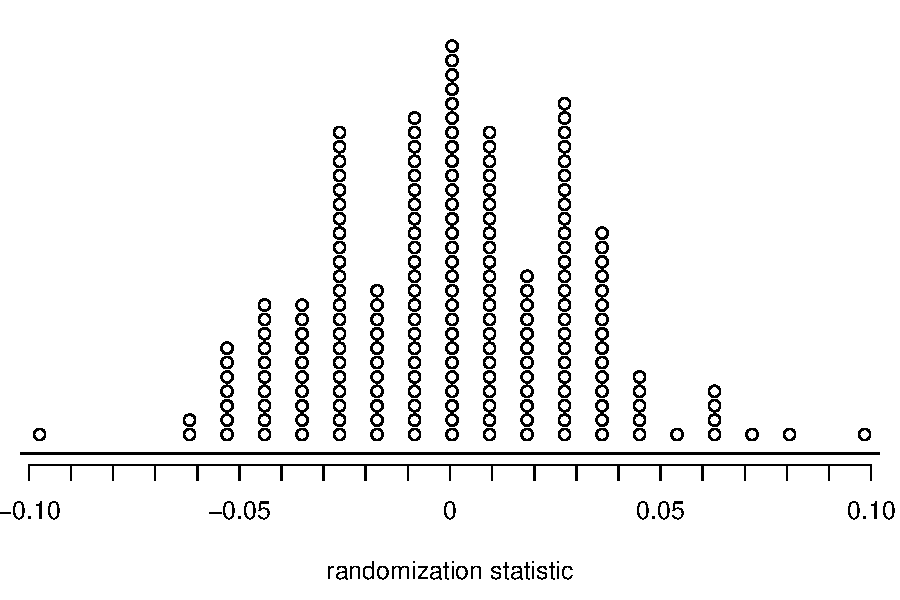
\includegraphics[width=0.9\textwidth]{figures/stroke/stroke}
\end{minipage}
\begin{minipage}[c]{0.3\textwidth}
\soln{Each dot represents a simulated difference between the proportions of strokes between the treatment and control groups}
\end{minipage}

\vfill

\pagebreak

%

\item \pts{2} Estimate the p-value based on this randomization test. Show all your work.

\soln{Proportion of simulations with $|\hat{p}_{sim,T} - \hat{p}_{sim,C}| \ge 0.09 = 2 / 200 = 0.01$}
$\:$ \\

\item \pts{4} What is the conclusion of the hypothesis test? Interpret your conclusion in context of the question?

\soln{p-value $<$0.05, reject $H_0$. The data provide convincing evidence to suggest that the proportion of patients with strokes is different between the treatment and control groups.}
$\:$ \\

\item \pts{3} What does a Type 1 error mean in context of this question?

\soln{Rejecting $H_0$ and determining that stroke rates are different for patients who receive and do not receive stents, when in reality those rates are the same. Or, deciding that stents have an effect on strokes, when in reality they don't.}
$\:$ \\

\item \pts{3} An introductory statistics student who reads this study remarks ``The results of this study do not suggest a causal relationship between stents and strokes because the difference between the stroke rates in the two groups could be due to aggressive medical management as well." Is this statement justified? Explain your reasoning.

\soln{No, patients are randomly assigned to these groups, hence this is an experiment, which allows us to draw causal conclusions. In addition, both groups receive the aggressive medical management so differences aren't due to that, but instead due to the only treatment different between the two groups: stents.}
$\:$ \\

\item \pts{3} Does it appear that stents are effective in \emph{reducing} the risk of strokes? Explain.

\soln{No, actually, there is a higher proportion of strokes in the treatment group. Proportion of strokes in the treatment group is significantly higher than the proportion of strokes in the control group (p-value - 0.005).}

\end{enumerate}

%

\pagebreak

\item The 2010 General Social Survey asked the question; ``Do you think the use of marijuana should be made legal, or not?" 48\% of the 1,259 respondents said it should be made legal.

\begin{enumerate}

\item \pts{2} Is the number ``48\%" a sample statistic or a population parameter? Explain.

\soln{Sample statistic, it's the observed proportion.}

\item \pts{5} Construct a 95\% confidence interval for the proportion of Americans who think marijuana should be made legal.
\soln{
\begin{align*}
\hat{p} &= 0.48 \\
0.48 &\pm 1.96 \sqrt{ \frac{0.48 * (1 - 0.48)}{1259} } \\
0.48 &\pm 1.96 * 0.014 \\
0.48 &\pm 0.0274 \\
(0.4526 &, 0.5074)
\end{align*}
}
\item \pts{3} Interpret this confidence interval in the context of this question.

\soln{We are 95\% confident that roughly 45.26\% to 50.74\% of Americans think marijuana should be legalized.}
$\:$ \\

\item \pts{4} A critic points out that this 95\% confidence interval is only accurate if the statistic follows a normal distribution, or if the normal model is a good approximation. Is this true for these data? Explain.

\soln{The number of successes (people who said marijuana should be legalized: $1259 * 0.48 = 604.32$) and failures (people who said it shouldn't be: $1259 * 0.52 = 654.68$) are both greater than 10, therefore the distribution of the statistic is expected to be nearly normal.}
$\:$ \\
$\:$ \\
$\:$ \\

\item \pts{3} A news piece on this study's findings states; ``Majority of Americans think marijuana should be legalized." Based on your confidence interval, is this news piece's statement justified? 

\soln{No, the interval contains 50\%, suggesting that the true population proportion could be just 50\% or even lower. Using this interval we wouldn't reject a null hypothesis where $p = 0.50$.}

\end{enumerate}

$\:$ \\

%

\pagebreak

\item The following histogram shows the distribution of IQ scores of fathers and mothers of a random sample of 36 students who were identified as ``gifted" soon after they turned four. Relevant summary statistics for both distributions are also provided.\footnote{Graybill, F.A. \& Iyer, H.K., (1994) Regression Analysis: Concepts and Applications, Duxbury, p. 511-6.}

\begin{minipage}[c]{0.5\textwidth}
\begin{center}
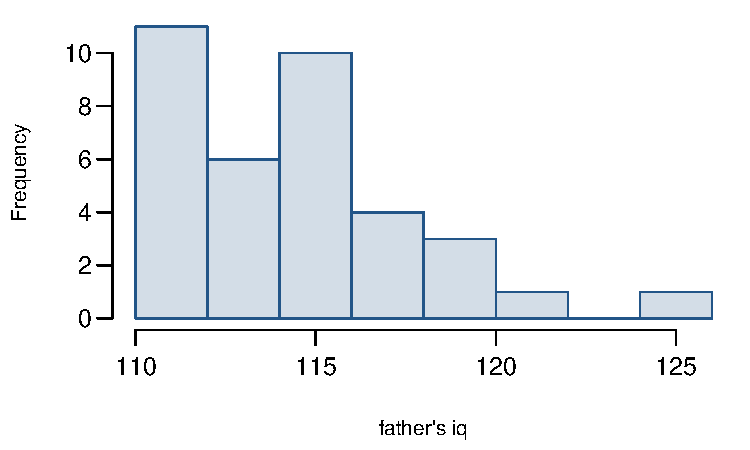
\includegraphics[width=0.7\textwidth]{figures/gifted/father_iq_hist}
{\footnotesize
\begin{verbatim}
   Min. 1st Qu.  Median    Mean 3rd Qu.    Max. 
  110.0   112.0   115.0   114.8   116.2   126.0 
\end{verbatim}
}
\end{center}
\end{minipage}
\begin{minipage}[c]{0.5\textwidth}
\begin{center}
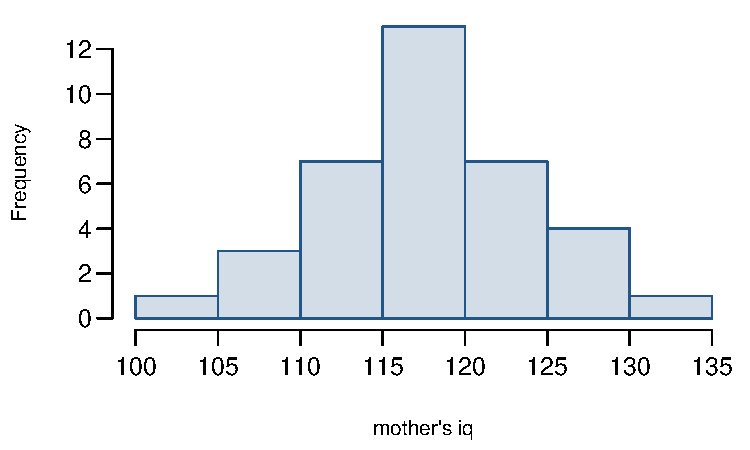
\includegraphics[width=0.7\textwidth]{figures/gifted/mother_iq_hist}
\end{center}
{\footnotesize
\begin{verbatim}
   Min. 1st Qu.  Median    Mean 3rd Qu.    Max. 
  101.0   113.8   118.0   118.2   122.2   131.0 
\end{verbatim}
}
\end{minipage}

\begin{enumerate}

\item \pts{3} Given below is a dot plot of the bootstrap distribution of means of \emph{200 bootstrap samples} taken from the original sample of differences between the IQ scores of father and mother of a child (father's IQ score - mother's IQ score).
\begin{center}
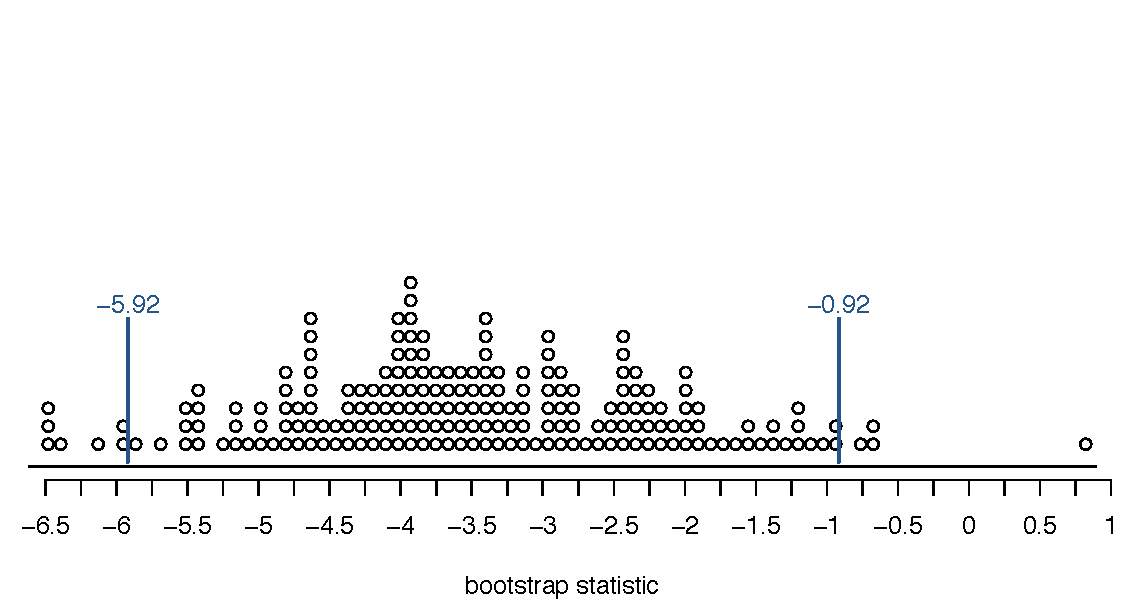
\includegraphics[width=0.9\textwidth]{figures/gifted/iqdiff_boot_soln}
\end{center}
Based on this distribution, estimate a 95\% confidence interval for the true average difference between the IQ scores of fathers and mothers of gifted children. Report the numerical values of the bounds of the confidence interval \emph{and} draw vertical lines indicating where they would fall on the plot.


\soln{Lower bound: any answer between -5.75 and -6 accepted. Upper bound: any answer between -0.75 and -1 accepted.\\
Exact: (-5.92, -0.92)}

\item \pts{3} Interpret this interval in context of this question. 

\soln{We are 95\% confident that the average IQ scores of fathers of gifted children are 5.92 to 0.92 points lower than their mothers' IQ scores.}

\vfill
\pagebreak

%

\item \pts{3} You overhear two researchers talking about this study and one of them says; ``This confidence interval shows that mothers of gifted children on average have significantly higher IQ scores than their fathers." Is this statement justified? Explain your reasoning.

\soln{Yes, the confidence interval doesn't include 0, and both bounds are negative, suggesting mothers of gifted children on average have significantly higher IQ scores than their fathers.}
$\:$\\
$\:$\\

\item \pts{4} A hypothesis test for testing for the \emph{difference} between the mean IQ scores of fathers and mothers of gifted children yields a p-value of 0.0098. Interpret the meaning of this probability in context of this research question.

\soln{Point estimate: $\bar{x}_F - \bar{x}_M = 114.8 - 118.2 = -3.4$\\
$\:$ \\
If in fact fathers and mothers of gifted children have on average the same IQ score, the probability of getting a sample of 36 gifted children where the difference between the average IQ scores of fathers and mothers is 3.4 points or more is 0.0098.}

\end{enumerate}
%

\pagebreak

\begin{center}
\textit{Answer questions \ref{countF} to \ref{countL} based on the information below.}
\end{center}
$\:$
\hrule
The following histogram shows the distribution of the ages (in months) at which a random sample of 36 childen first counted to 10 successfully. These children were identified as ``gifted" soon after they turned four.\footnote{Graybill, F.A. \& Iyer, H.K., (1994) Regression Analysis: Concepts and Applications, Duxbury, p. 511-6.}

\begin{minipage}[c]{0.5\textwidth}
\begin{center}
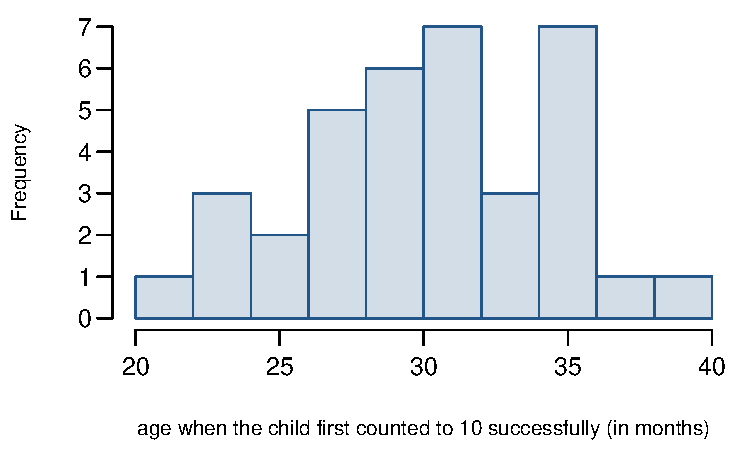
\includegraphics[width=\textwidth]{figures/gifted/count_hist}
\end{center}
\end{minipage}
\begin{minipage}[c]{0.5\textwidth}
\begin{center}
{\footnotesize
\begin{verbatim}
   Min. 1st Qu.  Median    Mean 3rd Qu.    Max. 
  21.00   28.00   31.00   30.69   34.25   39.00 
\end{verbatim}
}\end{center}
\end{minipage}
$\:$ \\
\hrule
$\:$

\item \pts{2} \label{countF} Which of the following is the correct set of hypotheses for testing if the average age at which gifted children fist count to 10 successfully is less than 32 months?

\begin{multicols}{2}
\begin{enumerate}
\item \solnMult{$H_0: \mu = 32$; $H_A: \mu < 32$}
\item $H_0: \mu = 32$; $H_A: \bar{x} < 30.69$
\item $H_0: p = 32$; $H_A: p < 32$
\item $H_0: \bar{x} = 32$; $H_A: \bar{x} < 32$
\end{enumerate}
\end{multicols}

\item \pts{2} Which of the following is an appropriate method for these data?

\begin{multicols}{2}
\begin{enumerate}
\item $\chi^2$ test of independence
\item $\chi^2$ test of goodness of fit
\item \solnMult{Z-test}
\item {T-test}
\end{enumerate}
\end{multicols}

\item \pts{2} The test statistic is calculated as -1.82. Which of the below ranges contain the p-value?

\begin{multicols}{2}
\begin{enumerate}
\item Less than 0.005
\item \solnMult{Between 0.025 and 0.05}
\item Between 0.05 and 0.1
\item Greater than 0.1
\end{enumerate}
\end{multicols}

\item \pts{2}  \label{countL} Which of the below is the best interpretation of the p-value for this hypothesis test?

\begin{enumerate}
\item Probability that gifted children successfully count to 10 at the average age of 32 months.
\item Probability that gifted children successfully count to 10 at the average age of less than 32 months.
\item \solnMult{Probability of getting a random sample of 36 gifted children where the average age at which they count to 10 successfully is 30.69 or less, if in fact the true mean is 32 months}
\item Probability of getting a random sample of 36 gifted children where the average age at which they count to 10 successfully is 30.69 or less, if in fact the true mean is less than 32 months
\end{enumerate}

\vfill

\pagebreak

%



%

\pagebreak

\begin{center}
\textit{Answer questions \ref{relaxF} to \ref{relaxL} based on the information below.}
\end{center}
$\:$
\hrule
The 2010 General Social Survey asked the question ``After an average work day, about how many hours do you have to relax or pursue activities that you enjoy?" to a random sample of 1,155 Americans. A 95\% confidence interval for the mean number of hours spent relaxing or pursuing activities they enjoy was	
\[ (1.38, 1.92) \]
\hrule
$\:$


\item \pts{2} \label{relaxF} Which of the following is a valid interpretation of this interval?
\begin{enumerate}
\item 95\% of all Americans spend between 1.38 to 1.92 hrs per day relaxing or pursuing activities they enjoy.
\item If a new survey with the same sample size were to be taken, there is a 95\% chance that the mean number of hours spent relaxing or pursuing activities enjoyed in the sample would be between 1.38 and 1.92.
\item We are 95\% confident that, were we to repeat this survey, the mean number of hours spent relaxing or pursuing activities they enjoy would be between 1.38 and 1.92.
\item \solnMult{We are 95\% confident that Americans spend an average of 1.38 to 1.92 hours per day  relaxing or pursuing activities they enjoy.} \\
\end{enumerate}

%

\item \pts{2} If the researchers who conducted this survey wanted to report a confidence interval with a \emph{larger} margin of error based on the same sample of 1,155 Americans, what would change?
\begin{enumerate}
\item the confidence level would go down
\item \solnMult{the confidence level would go up}
\item the confidence level would stay the same \\
\end{enumerate}

%

\item \pts{2} \label{relaxL} If a new survey were to be done with 2,500 Americans, which of the following would be true?
\begin{enumerate}
\item \solnMult{margin of error would be smaller}
\item margin of error would be larger
\item margin of error would be about the same
\end{enumerate}

%

\pagebreak

\item \pts{2} Does Weight Watchers work? Researchers randomly divided 500 people into two equal-sized groups. One group spent 6 months on the Weight Watchers program. The other group received a pamphlet about controlling portion sizes. At the beginning of the study, the average difference in weights between the two groups was approximately 0. After the study, the average difference was about 8 pounds. The Weight Watchers group had the lower average weight. To test whether an average difference of 8 pounds could be due to chance, a statistician writes everyone's end-of-diet weight on an index card. He shuffles these cards together, and then deals them into two equal-sized groups. Which of the following best describes the expected result?

\begin{enumerate}
\item The average difference between the two stacks of cards will be about 8 pounds.
\item \solnMult{The average difference between the two stacks of cards will be about 0 pounds.}
\item If Weight Watchers was effective, the average difference between the two stacks of cards will be more than 8 pounds. \\
\end{enumerate}

%

\vspace{2cm}

\item \pts{7} Answer the following true / false questions. Each question is worth 1 point.
\begin{enumerate}[(a)]
\vspace{3mm} \item ( \solnMult{T} / F ) With large sample sizes even small differences between the null value and the point estimate, also called the effect size, can be statistically significant.
\vspace{3mm} \item ( \solnMult{T} / F ) If you found $\chi^2=10$ and df=5 you would fail to reject $H_0$ at 5\% significance level.
\vspace{3mm} \item ( T / \solnMult{F} ) A cutoff of $\alpha = 0.05$ is the ideal value for all hypothesis tests.
\vspace{3mm} \item ( \solnMult{T} / F ) We should be concerned about the independence of observations in a sample if we sample more than 10\% of the population without replacement.
\vspace{3mm} \item ( T / \solnMult{F} ) If the p-value is sufficiently large you can reject $H_A$.
\vspace{3mm} \item ( T / \solnMult{F} ) Power of a test and the probability of making a Type 1 error are complements.
\vspace{3mm} \item ( \solnMult{T} / F ) The equivalent confidence level for a two-sided hypothesis test with $\alpha = 0.05$ is 95\%.
\vspace{10mm}
\end{enumerate}

\end{enumerate}
%
%
\end{document}